\documentclass[11pt,a4paper]{article}
\usepackage[utf8]{inputenc}
\usepackage[T1]{fontenc}
\usepackage[french]{babel}
\usepackage[margin=1.4cm]{geometry}
\usepackage{amsmath}
\usepackage{xcolor}
\usepackage{hyperref}
\usepackage{enumitem}
\usepackage{graphicx}
\usepackage{helvet}

\renewcommand{\familydefault}{\sfdefault}

% --- PALETTE DE COULEURS ---
\definecolor{primary}{HTML}{0E2A47}
\definecolor{secondary}{HTML}{2563EB}
\definecolor{textdark}{HTML}{1E293B}
\definecolor{textgray}{HTML}{64748B}

\color{textdark}

\hypersetup{
    colorlinks=true,
    linkcolor=secondary,
    urlcolor=secondary
}

\newcommand{\cvsection}[1]{%
  \vspace{0.65em}%
  {\color{primary}\large\bfseries\uppercase{#1}}\\[0.1em]%
  {\color{secondary}\rule{\linewidth}{1pt}}%
  \vspace{0.25em}%
}

\setlist[itemize]{left=1em, label=\textcolor{secondary}{\small$\bullet$}, itemsep=0.15em, parsep=0pt, topsep=0.15em}

\pagestyle{empty}

\begin{document}

% --- EN-TÊTE ---
\begin{minipage}[c]{0.72\textwidth}
    {\Huge \textbf{\color{primary}Thélio Olivier Geiser}} \\[0.25em]
    {\large \color{secondary}\bfseries Étudiant en 2\textsuperscript{e} année de Génie Mécanique à l'EPFL} \\[0.4em]
    {\small \color{textdark}
    La Tour-de-Peilz, Suisse \quad|\quad +41 78 727 10 57 \quad|\quad \href{mailto:thelio.geiser@gmail.com}{thelio.geiser@gmail.com}
    }
\end{minipage}%
\hfill
\begin{minipage}[c]{0.24\textwidth}
    \begin{flushright}
        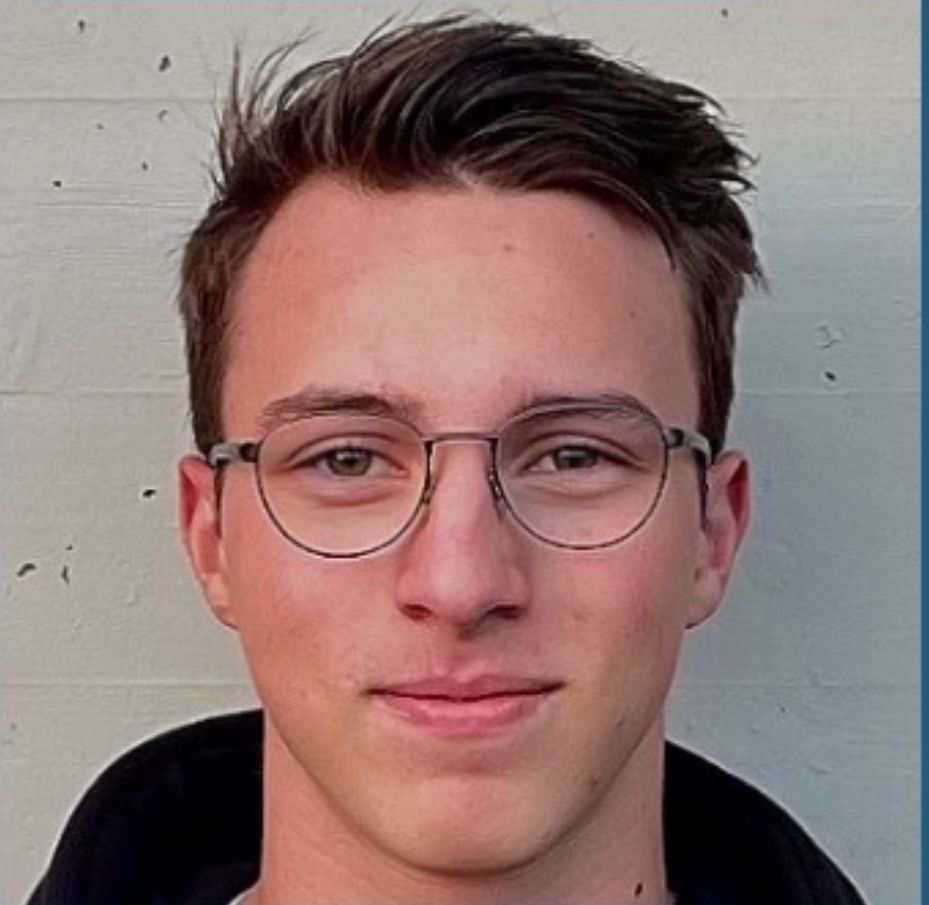
\includegraphics[width=2.8cm,height=3.6cm,keepaspectratio]{WhatsApp Image 2025-08-21 à 11.13.45_9a0f3007.jpg}
    \end{flushright}
\end{minipage}

\vspace{0.2em}

% --- PROFIL ---
\cvsection{Profil}
Étudiant en \textbf{2\textsuperscript{e} année de Génie Mécanique à l'EPFL}, j'allie une approche d'ingénierie orientée conception mécanique, simulation (FEA) et fabrication à de solides compétences en \textbf{développement web} et \textbf{administration système (Docker, Linux)}. Habitué à mener des projets techniques de bout en bout, du dimensionnement analytique au déploiement.

% --- FORMATION ---
\cvsection{Formation}

\noindent\textbf{École Polytechnique Fédérale de Lausanne (EPFL)} \hfill {\color{textgray}\small 2024 -- Présent} \\
\textit{Bachelor en Génie Mécanique — 2\textsuperscript{e} année} \\[0.3em]

\noindent\textbf{Gymnase de Burier} – La Tour-de-Peilz, Suisse \hfill {\color{textgray}\small Obtenu en 2024} \\
\textit{Maturité suisse, Option spécifique : Applications des Mathématiques et Physique}

% --- PROJETS & DISTINCTIONS ---
\cvsection{Projets \& Distinctions}

\noindent\textbf{1\textsuperscript{re} place — Mécathon EPFL $\times$ Dassault Systèmes} \hfill {\color{textgray}\small Novembre 2026} \\
\textit{Junior Entreprise EPFL — Conception d'une pédale d'accélérateur Formula Student en 24h (Binôme)}
\begin{itemize}
    \item Conception CAO complète sous \textbf{3DEXPERIENCE (CATIA)} d'un ensemble de \textbf{441,2 g} ($< 450\text{ g}$), intégrant une structure en treillis de Warren (Al 6061/7075), une plaque CFRP et une double redondance (capteurs APPS et ressorts à gaz).
    \item Dimensionnement cinématique (course de $20,5^\circ$, effort linéaire progressif) et validation structurelle par \textbf{éléments finis (FEA)} et calculs analytiques (critères de Von Mises et Tsai-Hill, $FoS \ge 1,64$).
\end{itemize}

\noindent\textbf{Développement de plateformes web associatives} \hfill {\color{textgray}\small 2025 -- Présent} \\
\textit{Commission Romande de Chimie (CRC) \& Société Suisse des Professeurs de Sciences Naturelles (SSPSN)}
\begin{itemize}
    \item Conception, développement et déploiement de portails web modernes et d'outils de gestion de contenu pour des associations d'enseignants suisses (Astro, JavaScript, architecture modulaire).
\end{itemize}

% --- COMPÉTENCES ---
\cvsection{Compétences}

\begin{description}[leftmargin=0pt, labelindent=0pt, itemsep=0.25em]
    \item[\textcolor{primary}{CAO \& Simulation :}] 3DEXPERIENCE, CATIA V5, Fusion 360, Simulation par éléments finis (FEA / Von Mises)
    \item[\textcolor{primary}{Programmation \& Calcul :}] Python, C, MATLAB, \LaTeX
    \item[\textcolor{primary}{Développement Web :}] HTML5, CSS3, JavaScript, Astro, React
    \item[\textcolor{primary}{DevOps \& Environnement :}] Docker, Linux
    \item[\textcolor{primary}{Langues :}] Français (\textit{natif}), Anglais (\textit{B2} — séjour de 6 mois au Canada), Allemand (\textit{B2} — séjour de 4 mois en Allemagne)
    \item[\textcolor{primary}{Permis :}] Permis de conduire Voiture (B) et Moto (A)
\end{description}

% --- EXPÉRIENCE PROFESSIONNELLE ---
\cvsection{Expérience Professionnelle}

\noindent\textbf{Employé polyvalent (extra)} – Funplanet, Rennaz \hfill {\color{textgray}\small Mars 2024 -- Août 2024}
\begin{itemize}
    \item Participation active à la logistique, à l'accueil client et aux opérations quotidiennes en environnement à forte affluence.
\end{itemize}

\noindent\textbf{Stagiaire} – De Pury Pictet Turrettini, Genève \hfill {\color{textgray}\small 2 semaines (2024)}
\begin{itemize}
    \item Numérisation, classification et archivage sécurisé de dossiers financiers confidentiels dans le respect strict des procédures.
\end{itemize}

% --- CENTRES D’INTÉRÊT ---
\cvsection{Centres d'intérêts}
\begin{itemize}
    \item \textbf{Mécanique \& Sports mécaniques :} Entretien mécanique moto, karting et intérêt marqué pour l'ingénierie automobile.
    \item \textbf{Condition physique :} Pratique régulière de la musculation et du fitness.
\end{itemize}

\end{document}